%%%%%%%%%%%%%%%%%%%%%%%%%%%%%%%%%%%%%%%%%%%%%%%%%%%%%%%%%%%%%%%%%%%%
\chapter{Results}
\label{results}
\graphicspath{{chapter_05/figures}{chapter_05/tables}}
%%%%%%%%%%%%%%%%%%%%%%%%%%%%%%%%%%%%%%%%%%%%%%%%%%%%%%%%%%%%%%%%%%%%

This chapter presents the findings of the research carried out in this thesis to assess how effectively different forecasting methodologies (i.e., rainfall-based forecasts or data-driven approaches combining hydro-meteorological data) identify areas at risk of flash floods, and what predictability we should expect from both systems.

The analysis progresses through three interconnected components that collectively establish the current capabilities and future potential of the above-described flash flood prediction systems. 

Our research starts with the flash-flood-focused evaluation of short- and long-range rainfall estimates from ERA5-ecPoint. These post-processed estimates have been shown to represent better than ERA5 extreme rainfall estimates at point-scale, making it an ideal candidate for establishing baseline predictive capabilities across diverse geographical and climatological contexts \citep{Pillosu_2025a}. While such improvement in the prediction of localised extreme rainfall should enable improved detection of areas at risk of flash floods, the flash-flood-focused assessment is fundamental to determine a baseline to compare more sophisticated prediction systems, such as the data-driven approach that combines hydro-meteorological parameters.

Building upon this foundation, the second analytical component introduces a data-driven approach integrating hydro-meteorological parameters to enhance flash flood prediction. Whilst rainfall's magnitude, duration, and location are critical factors, flash flood occurrence depends upon complex interactions between meteorological forcing and catchment characteristics, including antecedent soil moisture conditions, topographical features, and land cover. The data-driven model developed herein incorporates these factors to capture the nonlinear relationships that govern flash flood generation, moving beyond purely meteorological prediction towards a more holistic hydro-meteorological framework.

The temporal dimension of forecast skill forms the third pillar of this analysis. Understanding how predictive capability degrades with increasing lead time is paramount for operational implementation, as it determines the practical warning times available to emergency managers and at-risk communities. This temporal analysis extends up to 5 days ahead, encompassing the full range of lead times relevant to flash flood preparedness and response activities. Day 1 forecasts would be used to activate emergency operation centres, pre-position resources in high-risk areas, and issue public warnings through media channels. Day 2-3 forecasts would be used to support broader preparedness activities, including mobilising regional resources, implementing precautionary evacuations in highly vulnerable areas, and allowing businesses and schools to adjust operations. Day 4-5 forecasts, whilst containing greater uncertainty, permit strategic planning such as adjusting reservoir operations, preparing emergency shelters, and enabling voluntary protective actions by residents, and although forecast skill diminishes at these lead times, the information remains valuable for initial situational awareness. By quantifying skill degradation across different forecast horizons, this analysis establishes realistic expectations for early warning systems and identifies the temporal windows within which different decision-making processes can be reliably supported.

Throughout this thesis, the flash-flood-focused verification framework described in section \ref{flash_flood_focused_verification_framework} has been applied to both rainfall-based and data-driven forecasts of areas at risk of flash floods to ensure comparability across approaches and lead times. The study utilises observational flash flood records from NOAA's Storm  Event Database across the contiguous US (CONUS), validated against ERA5-ecPoint rainfall forecasts and the data-driven hydro-meteorological predictions. Performance metrics include frequency bias and reliability diagrams to assess forecasts' reliability, and ROC curves and the estimation of the areas under the ROC curves to assess the predictions' discrimination ability. 

The results presented in the subsequent sections document the performance of both rainfall-based and data-driven hydro-meteorological forecasts. Section \ref{verif_rainfall_based_fc} shows the baseline verification results for the prediction of areas at risk of flash floods based using only ERA5-ecPoint short- and long-range rainfall predictions. Section \ref{verif_data_driven_short_fc} shows that the data-driven approach combining hydro-meteorological parameters yields statistically significant improvements in prediction skill, with particularly notable gains in discrimination ability as seen in the provided ROC curves. Section \ref{verif_data_driven_long_fc} shows that the predictive skill of the data-driven forecasts extends to day 5 with my better discrimination ability than its only rainfall-based counterpart. Section \ref{verif_case_study} shows a selection of flash flood events to illustrate the approaches' capacity to identify areas at risk of flash floods (in the US and around the world). Hence, the findings detailed in this chapter contribute to understanding how effectively current technologies can support flash flood warning systems.



%%%%%%%%%
\section{Assessment of rainfall-based predictions of areas at risk of flash floods}
\label{verif_rainfall_based_fc}

\subsection{Overall verification scores: frequency bias and area under the ROC curve}

\begin{figure}[htbp]
\centering
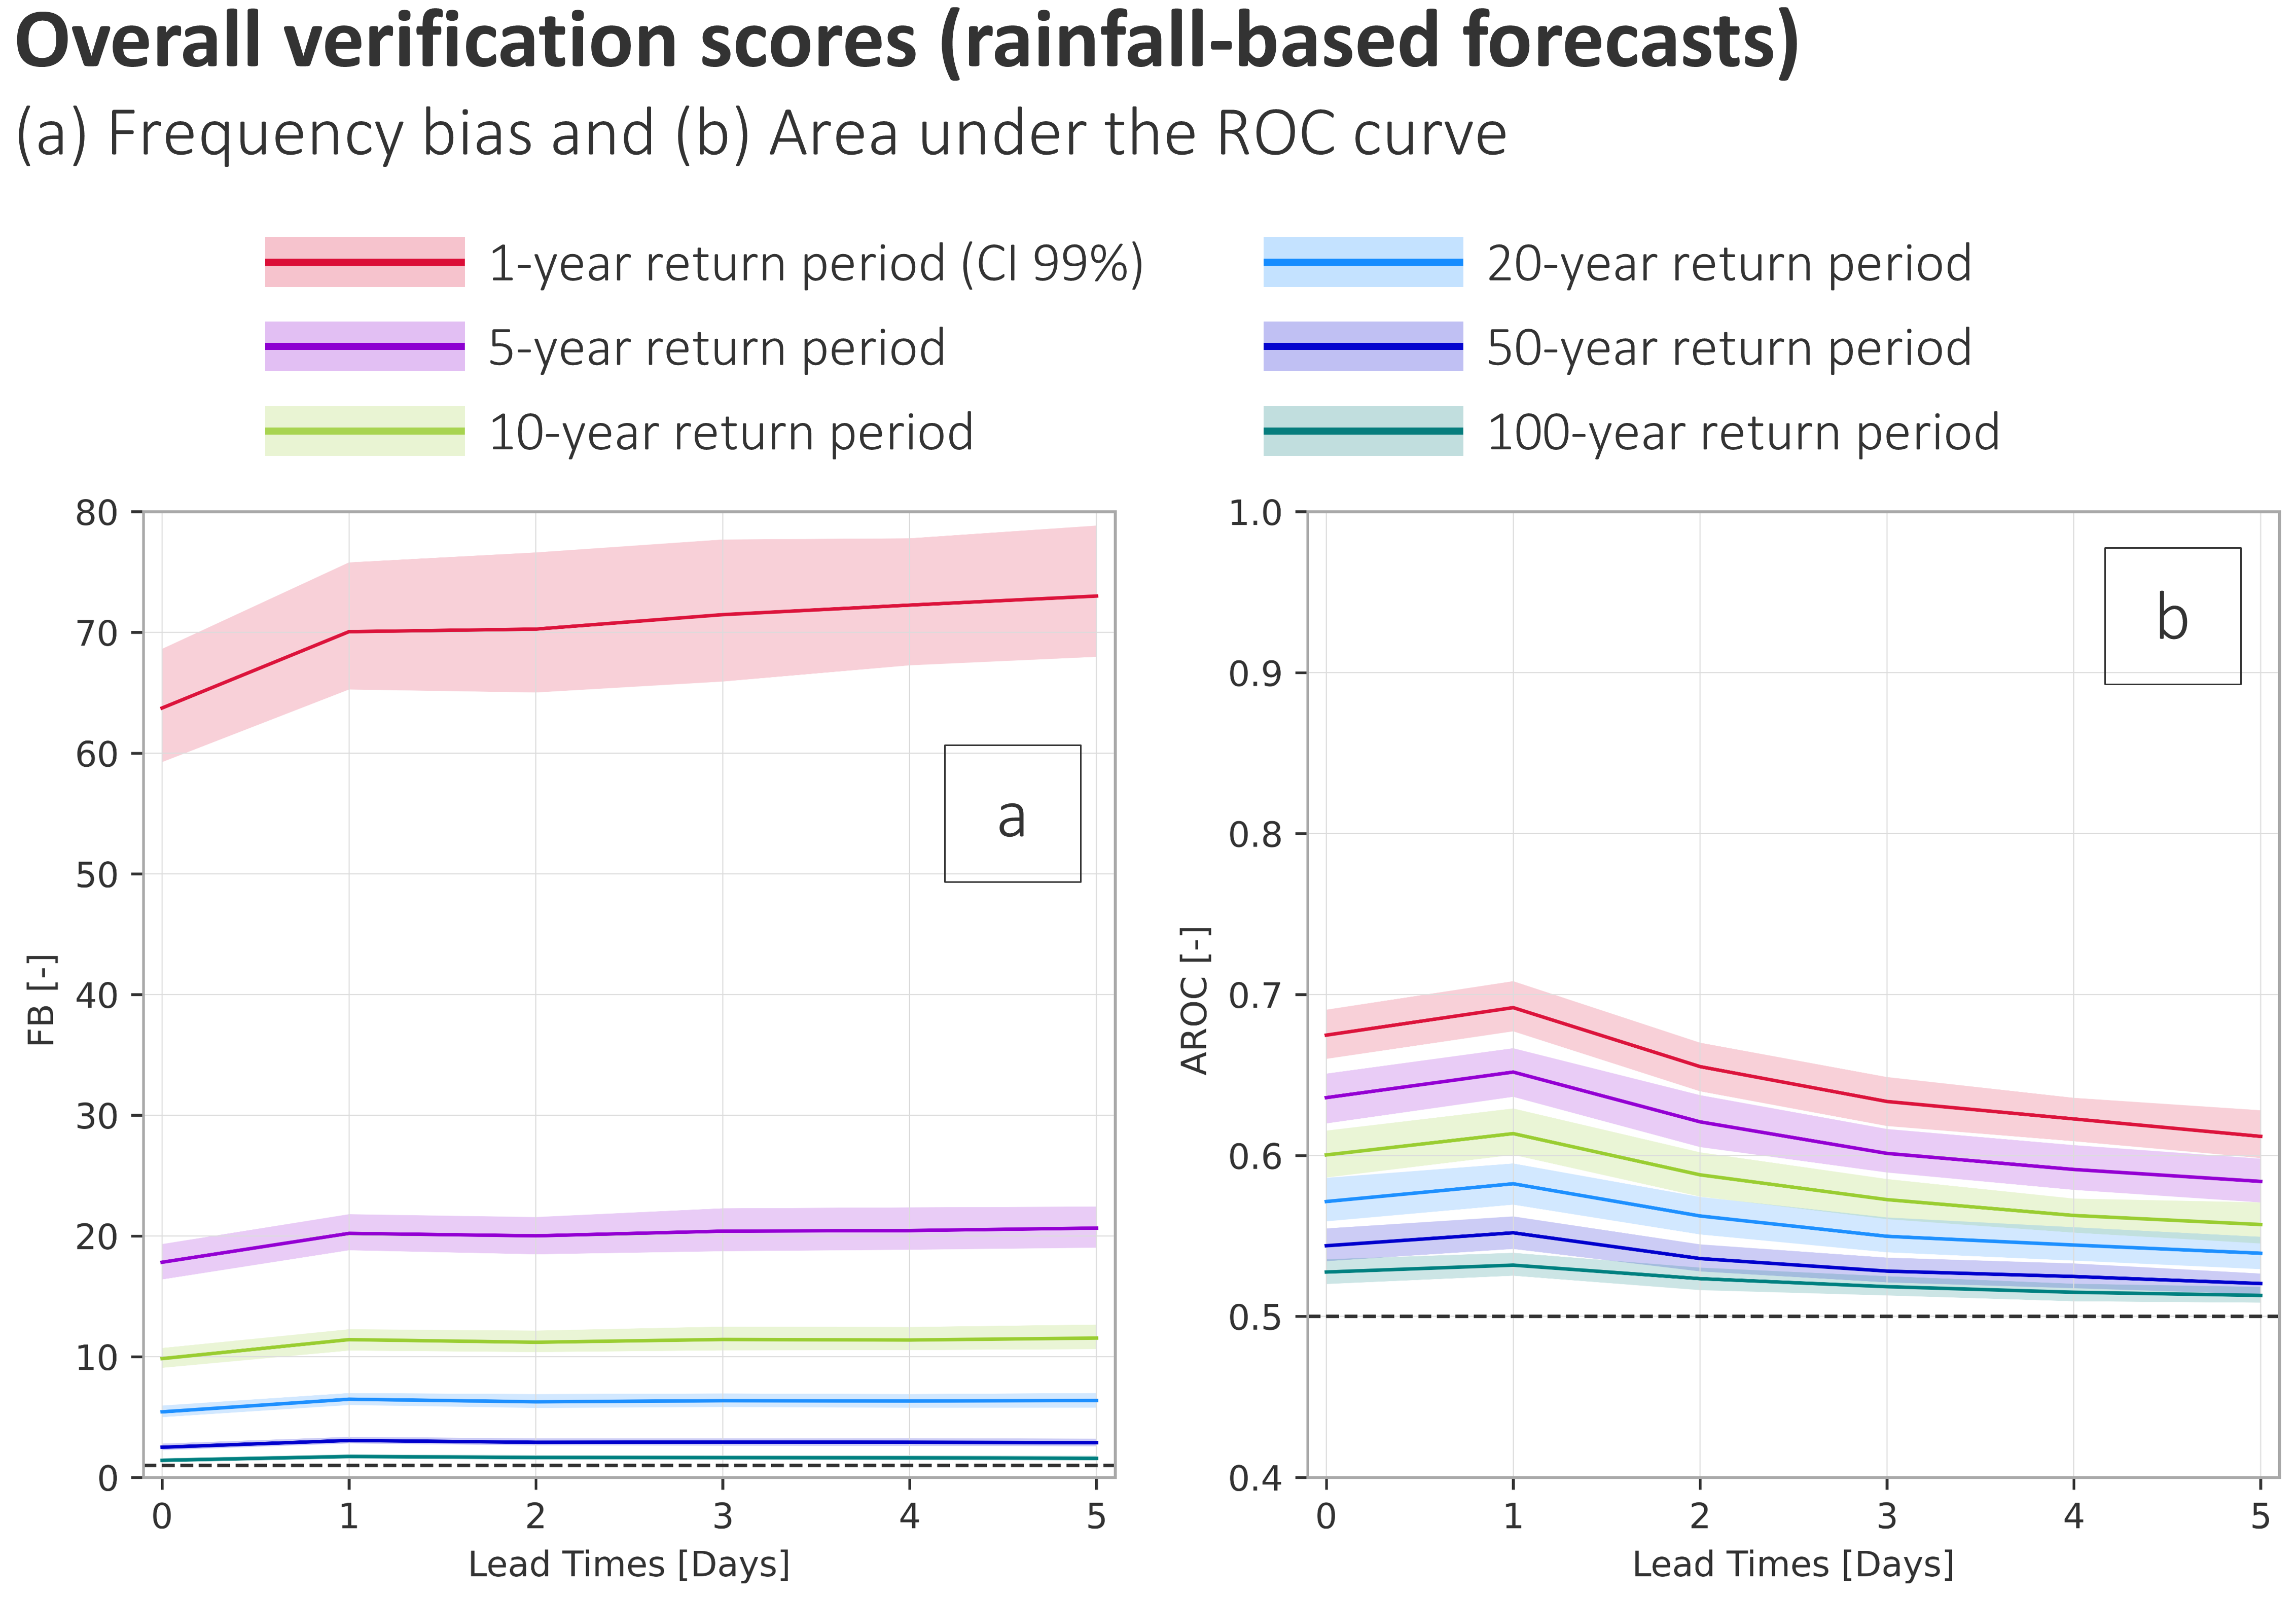
\includegraphics[width=\textwidth]{chapter_05/figures/rainfall_based_ff_verif_overall_scores.png}
\caption{\textbf{Overall verification scores for the rainfall-based forecasts of areas at risk of flash flood.} Panel (a) shows the frequency bias (solid lines) for 1-year (in red), 5-year (in purple), 10-year (in light green), 20-year (in cyan), 50-year (in blue), and 100-year return period (in green). The corresponding shaded areas represent the confidence intervals at 99\% confidence level. The inset box contains a zoomed-in version of panel (a) to show better the frequency bias values close to 1 (representing perfect bias). Panel (b) shows the area under the ROC curve.}
\label{fig:rainfall_based_ff_verif_overall_scores}
\end{figure}


\subsection{Discrimination ability}

All forecasts for rainfall events exceeding the 1-year return period threshold (Figure \ref{fig:rainfall_based_ff_roc_1rp}) exhibit a discrimination ability superior to random chance, as the curves are above the diagonal reference line. A systematic degradation in discrimination ability is observed with increasing lead time, with the Area Under the ROC Curve (AROC) values ranging from 0.675 for the short-range forecasts (Figure \ref{fig:rainfall_based_ff_roc_1rp}a) to 0.612 (\sim9\% reduction) for t+120 (day 5, Figure \ref{fig:rainfall_based_ff_roc_1rp}f). Despite such a reduction, the forecasts show a good discrimination ability throughout the forecast horizon. Day 1 forecasts (t+24) show a higher discrimination ability than the short-range forecasts, and only from day 2 forecasts (t+48), the discrimination ability of the long-range forecasts goes below that of the reanalysis. The relatively narrow confidence intervals (at 99\% confidence level) suggest that the differences in skill between forecast configurations are statistically meaningful at the considered confidence level.

\begin{figure}[htbp]
\centering
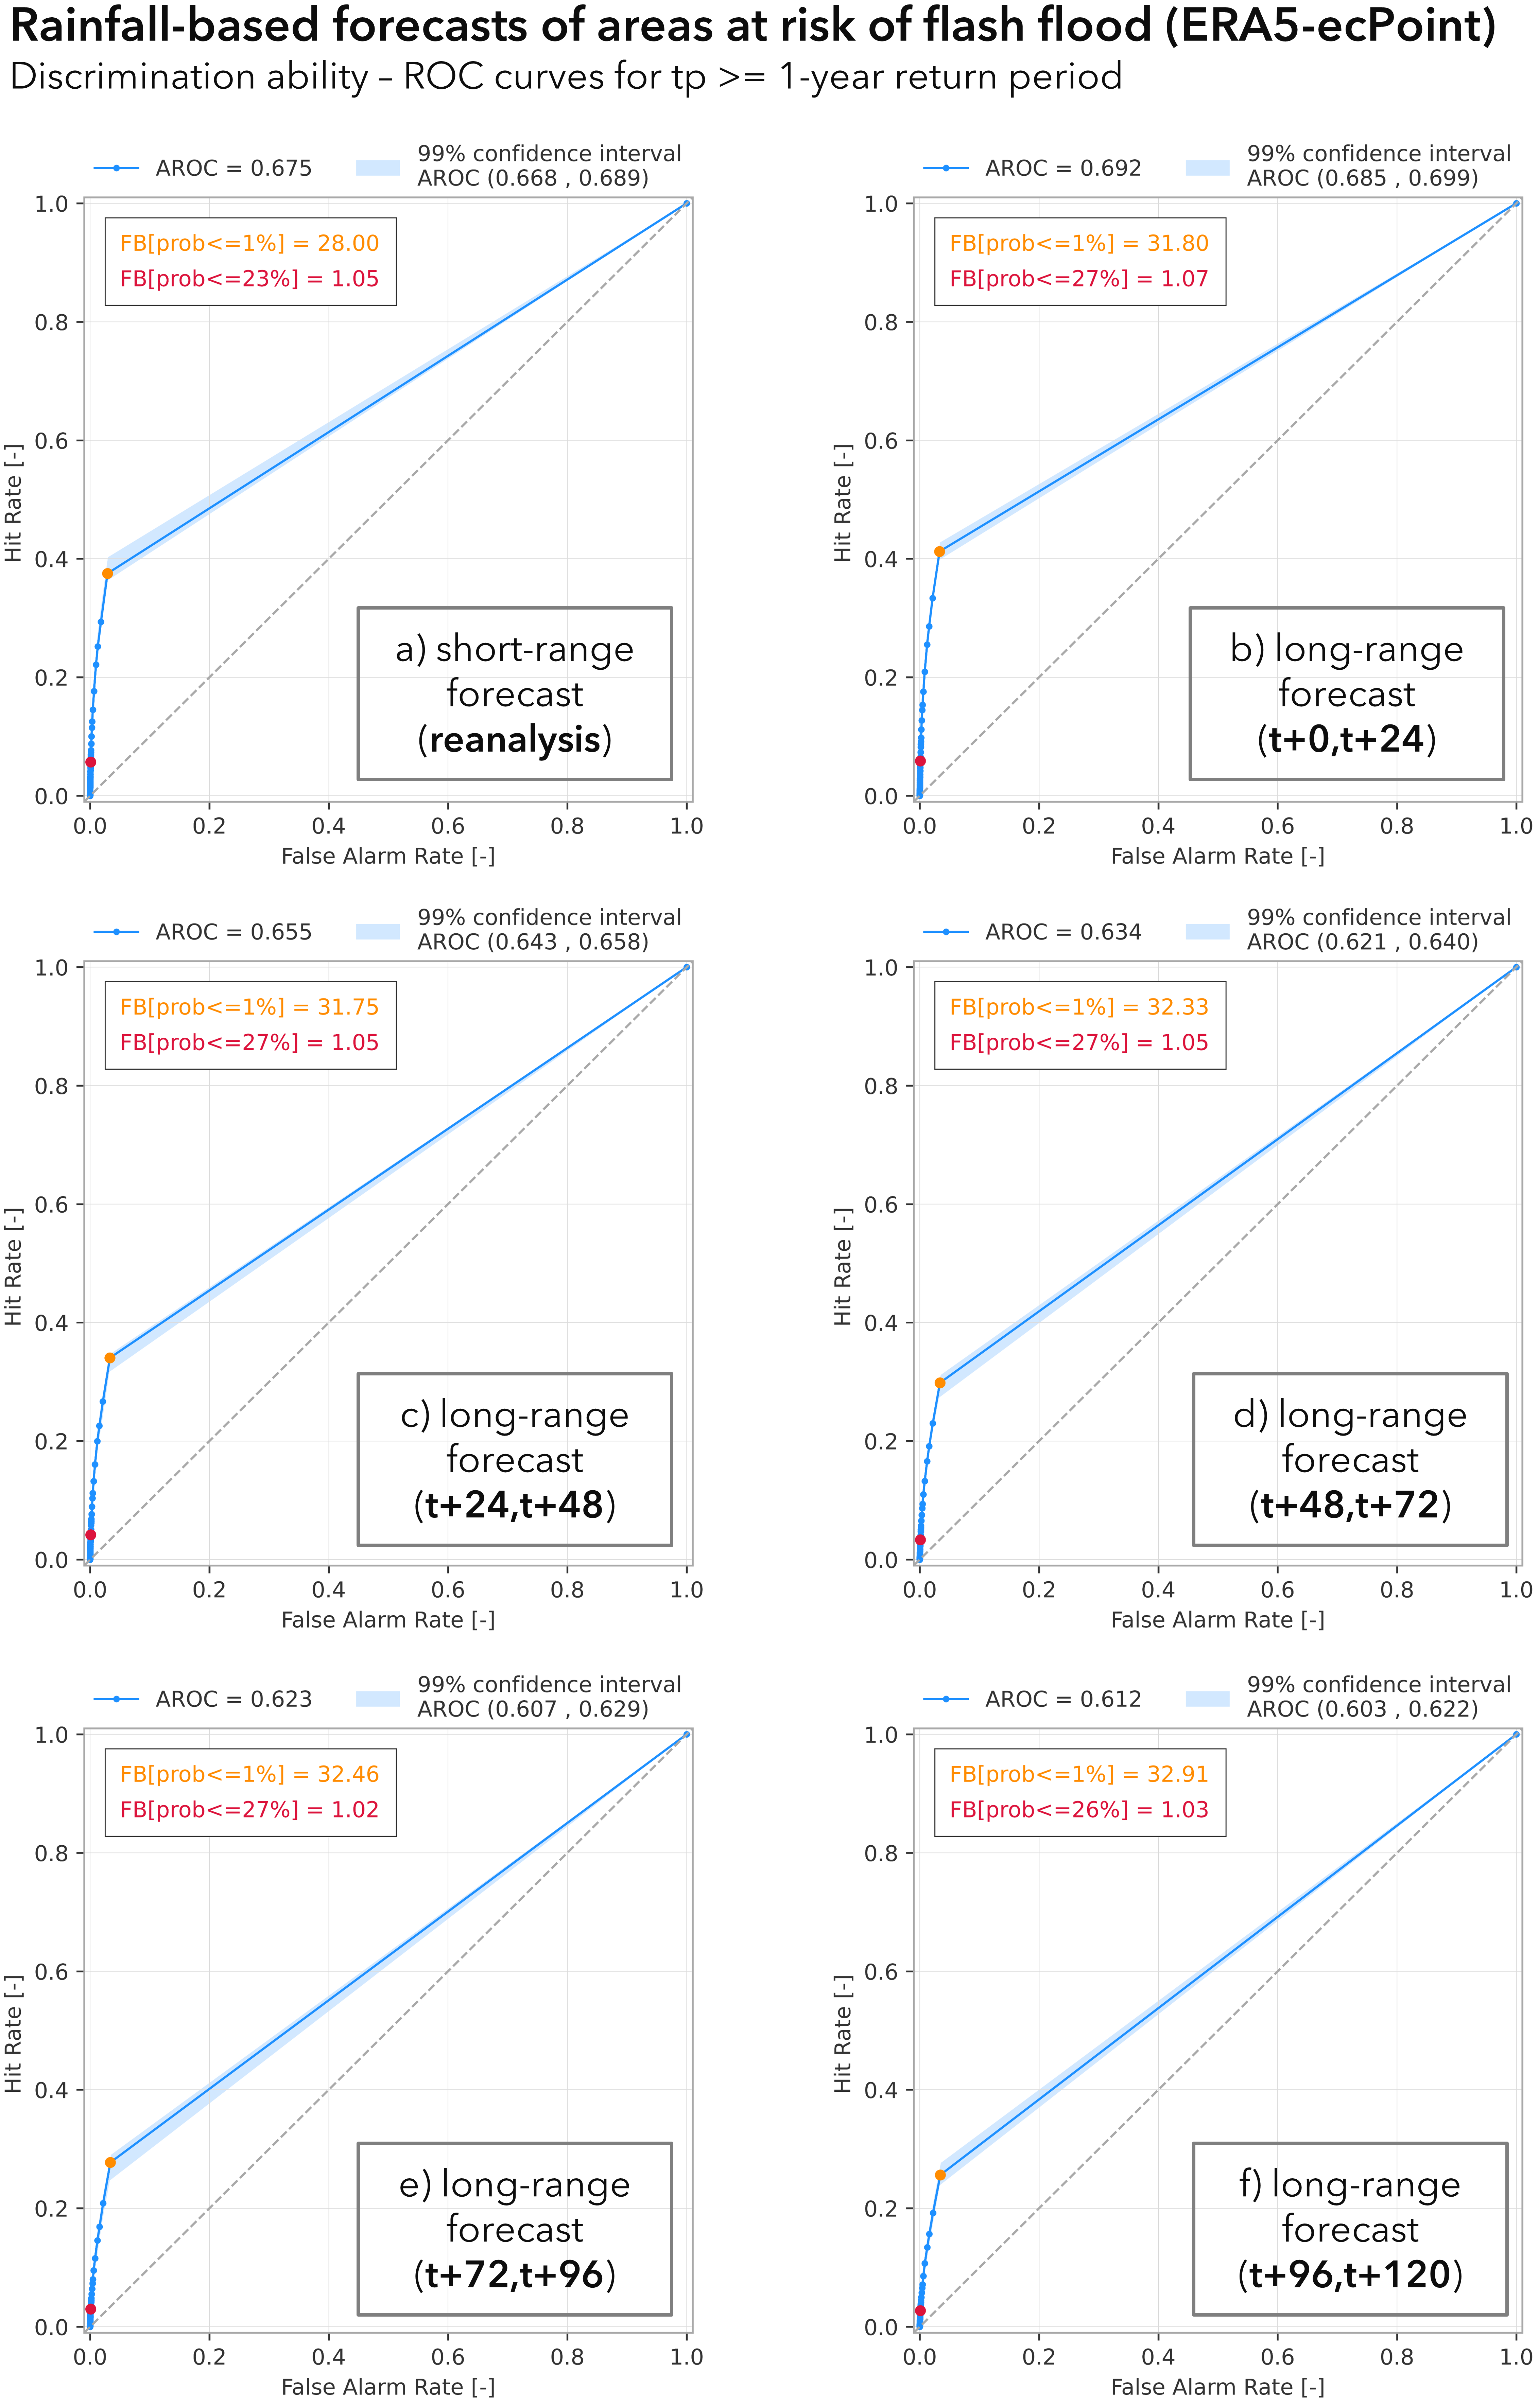
\includegraphics[width=\textwidth]{chapter_05/figures/rainfall_based_ff_roc_1rp.png}
\caption{\textbf{ROC curves for tp >= 1-year return period for the rainfall-based forecasts of areas at risk of flash floods built with ERA5-ecPoint.} Panel (a) shows the ROC curve (blue solid line) for the short-range predictions together with the confidence intervals (blue shaded area) at 99\% confidence level. Panels (b) to (f) refer to the long-range forecasts, for accumulation periods ending in t+24, t+48, t+72, t+96, and t+120, respectively. The pink dots refer to the probability threshold at which the frequency bias has the closest value to 1 (i.e., perfectly reliable forecast), while the orange dot shows the value of the frequency bias for the lowest probability threshold available in ERA5-ecPoint (i.e., the 99th percentile).}
\label{fig:rainfall_based_ff_roc_1rp}
\end{figure}

The pink dot in Figure \ref{fig:rainfall_based_ff_roc_1rp}a shows that perfect reliability (i.e. frequency bias equal to 1) is reach for probabilities <= 23\%. For the long-range forecasts, the probability thresholds at which perfect reliability is achieved is compatible to the short-range, being 27\% for all the lead times except t+120 which is 26\%. The frequency bias for the lowest probability threshold (i.e. 99th percentile or probability threshold equal to 1\%) in the short-range forecasts equals to 28. The frequency biases for the long-range forecasts are similar, falling between 31 and 33. 

Similar results are obtained for the 5-, 10-, 20-, 50-, and 100-year return periods.


\subsection{Reliability}

All forecasts for rainfall events exceeding the 1-year return period threshold (Figure \ref{fig:rainfall_based_ff_roc_1rp}) exhibit a systematic overprediction across all lead times, as shown by the reliability diagram being below the diagonal line. This indicates that when the model predicts a given probability, the observed frequency of flash flood events is consistently lower. For example, when the forecasts indicate a 50\% chance of having a flash flood event, the observed frequency ranges from \sim10\% in the short-range forecasts (Figure \ref{fig:rainfall_based_ff_roc_1rp}a), and between 10\% (for t+24, Figure \ref{fig:rainfall_based_ff_roc_1rp}b) and 2\% (t+120, Figure \ref{fig:rainfall_based_ff_roc_1rp}f) in the long-range forecasts. As seen in the ROC curves, the confidence intervals at 99\% are fairly narrow, suggesting that the differences between the reliability diagrams at different lead times are significant at the considered confidence level. However, the confidence levels increase with increasing forecast probabilities. As seen in the corresponding sharpness diagrams (inset boxes in all panels of Figure \ref{fig:rainfall_based_ff_roc_1rp}), such widening of the confidence intervals is likely due to the low number of forecasts issued with probabilities higher than ~25\% (when the total number of instances lies below 1000 samples). Such predominance of low probability forecasts suggests that the model (ERA5-ecPoint) rarely expresses high confidence in extreme event occurrence. A notable characteristic of all the reliability diagrams in the Figure \ref{fig:rainfall_based_ff_roc_1rp} is the sharp increase in observed frequency for the highest probability bins (i.e. 80\% to 100\%). This steep rise suggests that when the model does issue high probability forecasts, these correspond to genuinely extreme events, though such forecasts remain infrequent.

\begin{figure}[htbp]
\centering
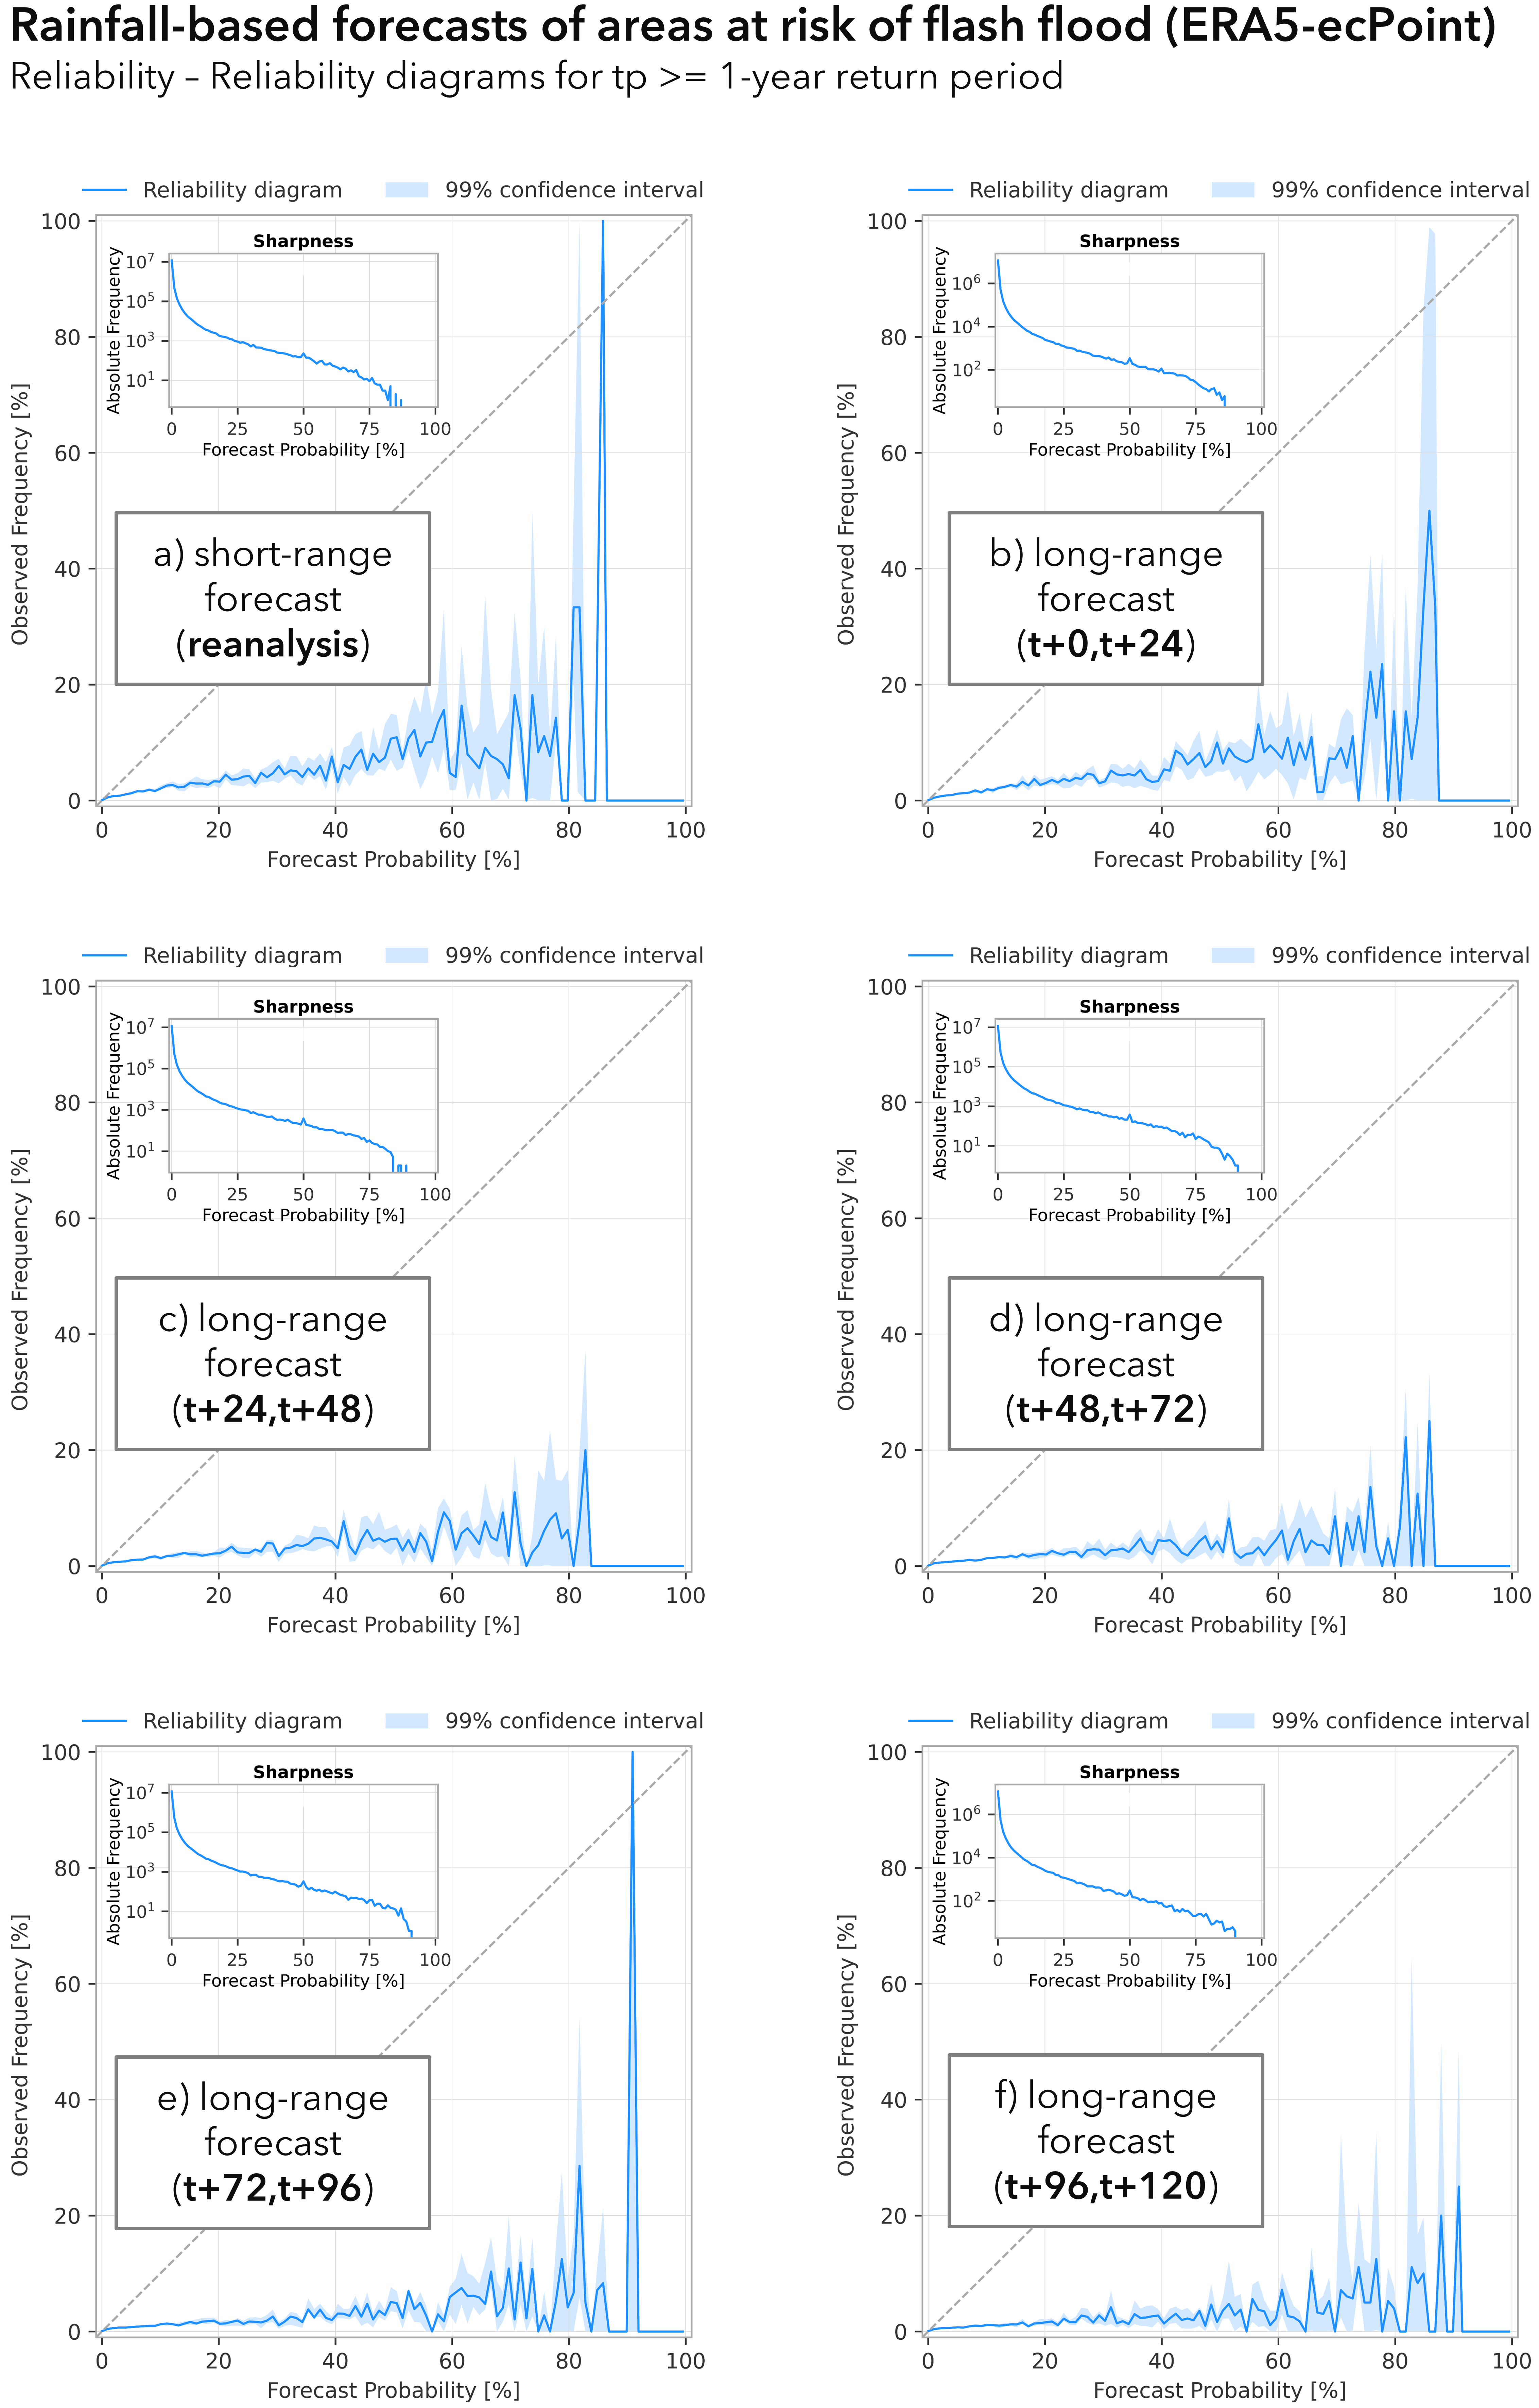
\includegraphics[width=\textwidth]{rainfall_based_ff_rel_diag_1rp.png}
\caption{\textbf{Reliability diagrams for tp >= 1-year return period for the rainfall-based forecasts of areas at risk of flash floods built with ERA5-ecPoint.} Panel (a) shows the reliability diagram (blue solid line) for the short-range predictions together with the confidence intervals (blue shaded area) at 99\% confidence level. Panels (b) to (f) refer to the long-range forecasts for accumulation periods ending in t+24, t+48, t+72, t+96, and t+120, respectively. The inset boxes show the corresponding sharpness diagrams.}
\label{fig:rainfall_based_ff_roc_1rp}
\end{figure}

The temporal evolution from Figure \ref{fig:rainfall_based_ff_roc_1rp}a to f reveals subtle changes in the forecasts' reliability characteristics with increasing lead time. Whilst the general pattern of overprediction persists, from day 2 forecasts (t+48) results more squashed into a flat line over very small observed frequencies, indicating that even though the model issues forecasts with high probabilities of exceeding the 1-year return period at longer lead times with a similar frequency of the short-range forecasts and the day 1 (t+24) long-range forecast, such forecasts do not necessarily correspond to an observed flash flood event.

The reliability diagrams get closer to the diagonal line (indicating perfect bias) as we increase the rainfall threshold to identify the flash flood events. Perfect reliability is observed for rainfall events exceeding the 10-, 20-year, and 50-year return period with probabilities below 5\% at day 1 forecast (t+24) for the 10-, 20-year return period, and 10\% for the 50-year return period.



%%%%%%%%%
\section{Assessment of short-range data-driven hydro-meteorological predictions of areas at risk of flash floods}
\label{verif_data_driven_short_fc}

\subsection{Model training}

\subsection{Comparative performance analysis with the rainfall-based predictions}
\subsubsection{Discrimination ability}
\subsubsection{Reliability}

\subsection{Physical interpretation of the data-driven model behaviour}

\subsection{Extension of regional training to global application}


%%%%%%%%%
\section{Assessment of long-range data-driven hydro-meteorological predictions of areas at risk of flash floods}
\label{verif_data_driven_long_fc}

\subsection{Discrimination ability}

\subsection{Reliability}


%%%%%%%%%
\section{Catalogue of flash flood events}
\label{verif_case_study}